\section{Основы линейной и нелинейной оптики.}

\subsection{Материальное уравнение линейной среды.}
\hspace*{2mm}
В основе взаимодействия света со средой лежит элементарный процесс возбуждения атома или молекулы вещества световым полем и последующего переизлучения света возбужденной частицей. Характер этого взаимодействия зависит от соотношения между величиной напряженности поля световой волны Е и характерной напряженностью внутриатомного поля  $E_{atom}$, определяющего силы связи оптических электронов (т.е. внешних, наиболее слабо связанных электронов) с ядром атома вещества.
\\
\hspace*{2mm}
Например, для атома водорода это поле составляет $ E_{atom} = e/(4\pi\epsilon_{0}r_{h}^2) = 5\cdot10^{11} $В/м, для более тяжелых атомов $ E_{atom} = 10^{10} \dots 10^{11} $ В/м. Оценка поля Е световой волны в случае не лазерных источников свет дает величину $E \le 10^3$ В/м, т.е. $E<<E_{atom} $. При этом условии отклик атомного осциллятора на внешнее воздействие будет иметь линейный характер, а зависимость поляризованности Р = Р(Е) в случае изотропной среды может быть представлена в виде:
\begin{equation}\label{1:liner}
P(E) = \chi^{(1)}E
\end{equation}

где $ \chi^{(1)}$ – линейная восприимчивость среды, являющаяся безразмерной величиной и зависящая только от свойств среды.
Материальное уравнение ($\ref{1:liner}$) является одним из соотношений, на которых базируется линейная оптика.  Но оно справедливо только при условии $E << E_{atom} $, а во слех остальных случаях является лишь некоторым приближением. 
\\
В мощных лазерных пучках можно получить напряженности уже сравнимые с $E_{atom} $. В случае когда поле Е, оставаясь меньше $E_{atom} $, приближается к нему по величине, поляризованность среды Р = Р(Е) перестает быть линейной функцией поля Е, и в этом случае материальное уравнение ($\ref{1:liner}$) должно быть заменено на другое.

\subsection{Материальное уравнение нелинейной среды.} 
\hspace*{2mm}
Теория нелинейно-оптических явлений строится на основе материальных уравнений и уравнений Максвелла. Уравнения Максвелла для диэлектрической нейтральной немагнитной среды имеют вид
\begin{equation}\label{1:maxvel}
rot\vec{E} = - \frac{ 1 }{ c}\frac{\partial \vec{H} }{\partial t}
\hspace{20mm}
rot\vec{H} =  \frac{ 1 }{ c}\frac{\partial \vec{D} }{\partial t}
\hspace{20mm}
div\vec{H} = 0
\end{equation}
где $ \vec{D} = \vec{E} + 4\pi \vec{P}$. Из уравнений Максвелла вытекает волновое уравнение
\begin{equation}\label{1:rot_maxvel}
rot(rot\vec{E}) + \frac{ 1 }{ c^2 }\frac{\partial^2 \vec{E} }{\partial t^2} = - \frac{ 4\pi }{ c^2 }\frac{\partial^2 \vec{P} }{\partial t^2}
\end{equation}
которе в случае изотропной среды принимает вид
\begin{equation}\label{1:wave_eq}
\Delta\vec{E} - \frac{ 1 }{ c^2 }\frac{\partial^2 \vec{E} }{\partial t^2} =  \frac{ 4\pi }{ c^2 }\frac{\partial^2 \vec{P} }{\partial t^2}
\end{equation}
где $\vec{E}$ - напряженность электрического поля, а $\vec{P}$ - поляризация среды. Поляризация среды возникает под действием падающий световой волны и описывается материальным уравнением $\vec{P} = \vec{P}(\vec{E})$.
В анизотропном случае $\vec{P}(\vec{E})$ являеться тензорный величиной и может быть представлена в виде:
\begin{equation}\label{1:p_1}
P(E) = \chi^{(1)}E + \chi^{(2)}E^2 \chi^{(3)}E^3\dots
\end{equation}
Коэффициенты $\chi^{(m)}, m \ge 2$ при членах разложения называются нелинейными восприимчивостями m-го порядка и являются уже размерными величинами. При этом соответствующая величина $\chi^{(m)}$ пропорциональна концентрации атомов (молекул) в веществе и m-ой степени параметра. Это означает, что отклик среды на действие внешнего светового поля перестает быть линейным.  С математической точки зрения именно это обстоятельство (нелинейность материального уравнения) является причиной нарушения принципа суперпозиции для световых волн в нелинейной среде. Из уравнений (\ref{1:rot_maxvel}), (\ref{1:wave_eq}) и (\ref{1:p_1}) непосредственно вытекает возможность генерации оптических гармоник и других нелинейно-оптических эффектов.  Надо отметить, что среды, в которых достаточно учитывать только первых два члена в уравнении ($\ref{1:wave_eq}$), называют квадратично-нелинейными средами, а среды с тремя первыми членами - кубически-нелинейными. 

\subsection{Нелинейная поляризация.} 
\hspace*{2mm}
Часть поляризации среды, нелинейно зависящая от напряженности светового поля, называется нелинейной поляризацией.Выделяя в поляризации среды линейную и нелинейную компоненты, можно записать:
\begin{equation}\label{1:p_non_liner}
\vec{P} = \vec{P}_{liner} + \vec{P}_{nonliner}
\end{equation}
подставив уравнение  (\ref{1:p_non_liner}) в  (\ref{1:rot_maxvel}) получим волновое уравнение для анизотропной среды и нелинейной изотропной среды:
\begin{equation}\label{1:wave_eq2}
\Delta\vec{E} - \frac{ 1 }{ c^2 }\frac{\partial^2 \vec{E} }{\partial t^2} - \frac{ 4\pi }{ c^2 }\frac{\partial^2 \vec{P}_{liner}}{\partial t^2} =  \frac{ 4\pi }{ c^2 }\frac{\partial^2 \vec{P} _{nonliner}}{\partial t^2}
\end{equation}
Нелинейная поляризация среды является источником новых спектральных компонент поля (оптических гармоник, комбинационных частот и т. п.). Материальное уравнение вида  (\ref{1:wave_eq}), описывает изотропную нелинейную среду с безынерционным локальным откликом на световое поле. Аналогичное уравнение для анизотропной нелинейной диспергирующей среды является уже не только тензорным, но и имеет комплексную часть: 
\begin{equation}
\chi^{(m)} = Re(\chi^{(m)}) + iIm(\chi^{(m)})
\end{equation}
причем коэффициенты восприимчивости, входящие в данное уравнение, уже зависят от времени о координаты. Среды, обладающие таким свойством, называют средами с пространственной дисперсией. К их 
числу относятся некоторые типы кристаллов, а также плазма.

\subsection{Основные процессы и эффекты нелинейной оптики}
Физические причины, приводящие к появлению нелинейных оптических эффектов, достаточно многообразны. К ним можно отнести:
\begin{enumerate}
\item  Нелинейную рефракцию в оптически прозрачной среде, т.е. зависимость показателя преломления среды от амплитуды светового вектора;
\item  Нелинейный характер рассеяния света в среде при больших интенсивностях светового поля;
\item  Многофотонное поглощение интенсивного оптического излучения в веществе;
\item  Генерацию высших гармоник при переизлучении световой волны;
\item  Тепловые самовоздействия и др.
\end{enumerate}
\begin{figure}[h]
	\centering
	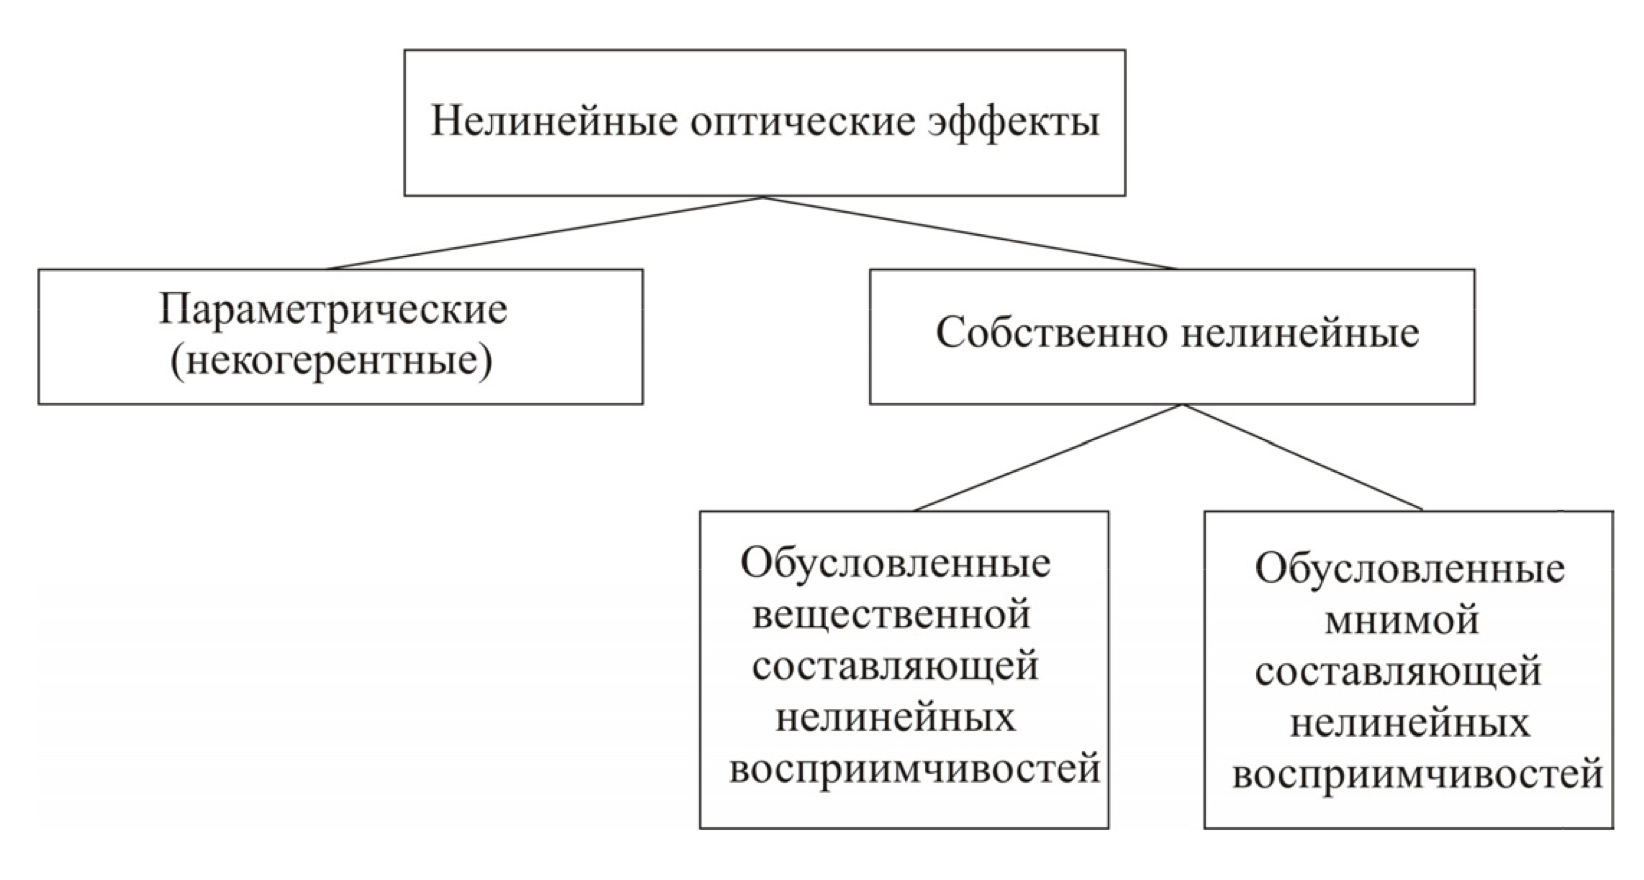
\includegraphics[width=0.7\linewidth]{images/classific.png}
	\caption{Классификация нелинейных оптических эффектов}
	\label{classific}
\end{figure}
К \textit{параметрическим явлениям} относятся:
\begin{enumerate}
\item   Электрооптический эффект, или эффект Поккельса (сообщение оптической анизотропии кристаллическим изотропным диэлектрикам без центра инверсии, помещенным в сильное однородное электрическое поле, при этом показатель преломления становится нелинейной функцией напряженности поля); является нелинейным эффектом второго порядка;
\item Эффект Керра (аналогичен эффекту Поккельса, но является нелинейным эффектом третьего порядка) и ряд других.
\end{enumerate}
К эффектам, \textit{обусловленным вещественной составляющей нелинейных восприимчивостей}, относятся:
\begin{enumerate}
\item  Эффекты генерации высших оптических гармоник, в частности, связанные с удвоением и утроением частоты света;
\item  Самовоздействие интенсивного светового пучка в нелинейных материалах (например, явление самофокусировки, при котором возникает перепад свойств среды в пучке и вне пучка, а его распространение приобретает волноводный, нитевидный характер, устраняющий геометрическую и дифракционную расходимость; при самофокусировке нарушается закон прямолинейного распространения света);
\item Оптический пробой среды, в основе которого лежит процесс качественного превращения прозрачной в сильно поглощающую среду с изменением агрегатного состояния при некотором значении интенсивности света;
\end{enumerate}
К эффектам, \textit{обусловленным мнимой составляющей нелинейных восприимчивостей}, относятся:
\begin{enumerate}
\item  Многофотонные процессы (фотоионизация и фотовозбуждение, гиперрассеяние света и другие), когда в элементарном акте взаимодействия света с атомом вещества участвует не один, а несколько фотонов; если мнимая составляющая линейной восприимчивости ответственна за однофотонные процессы, то мнимые составляющие восприимчивостей высших порядков – за многофотонные процессы;
\item  Вынужденное комбинационное рассеяние света, заключающееся в том, что интенсивное падающее излучение вызывает появление в оптической среде волны рассеянного стимулированного излучения на смещенных (комбинационных) частотах, характеристики которого имеют нелинейную зависимость от характеристик вынуждающего излучения;
\item Вынужденное рассеяние Мандельштама – Бриллюэна, при котором мощное световое излучение возбуждает в среде когерентные колебания молекул по закону бегущей волны, при этом происходит рассеяние света на образовавшейся периодической структуре (сверхзвуковой волне).
\end{enumerate}


\subsection*{Генерация второй оптической гармоники} 
Обсудим подробнее эффект удвоения частоты света в кристалле — генерации второй оптической гармоники. Данный эффект состоит в том, что под действием мощного лазерного излучения в нелинейном кристалле возникает излучение на удвоенной частоте.
\\
Пусть на квадратично-нелинейную среду воздействует монохроматическое поле с частотой $\omega$:
\begin{equation}\label{shg:e(t)}
A(t) = A\cos(\omega t)
\end{equation}
Тогда нелинейная поляризация второго порядка будет пропорциональна полю во второй степени:
\begin{equation}\label{shg}
P(t)^{(2)} = \chi^{(1)}E(t)^2 = \frac{1}{2}\chi^{(1)}A^2 + \frac{1}{2}\chi^{(1)}A^2\cos(2\omega t)
\end{equation}
Это значит, что поляризация будет иметь постоянную составляющую $ \frac{1}{2}\chi^{(1)}A^2$ , и переменную $\frac{1}{2}\chi^{(1)}A^2\cos(2\omega t)$, на удвоенной частоте $2\omega$. Первое слагаемое в (\ref{shg}) соответствует нелинейному процессу, который называется \textbf{оптическим выпрямлением}, а второе – \textbf{генерации второй гармоники}. 
\\
Происходит возбуждение волны поляризации на удвоенных частотах $2\omega_{1,2}$ (\textbf{генерация второй гармоники}, SGH), разностной $\omega_1 + \omega_2$(\textbf{генерация разностной частоты}, ГРЧ), суммарной $\omega_1 - \omega_2$ (\textbf{генерация суммарной частоты}, ГСЧ), и нулевой (\textbf{оптическое выпрямление}) частотах (рис. \ref{sghPictr}).
\begin{figure}[h]
	\centering
	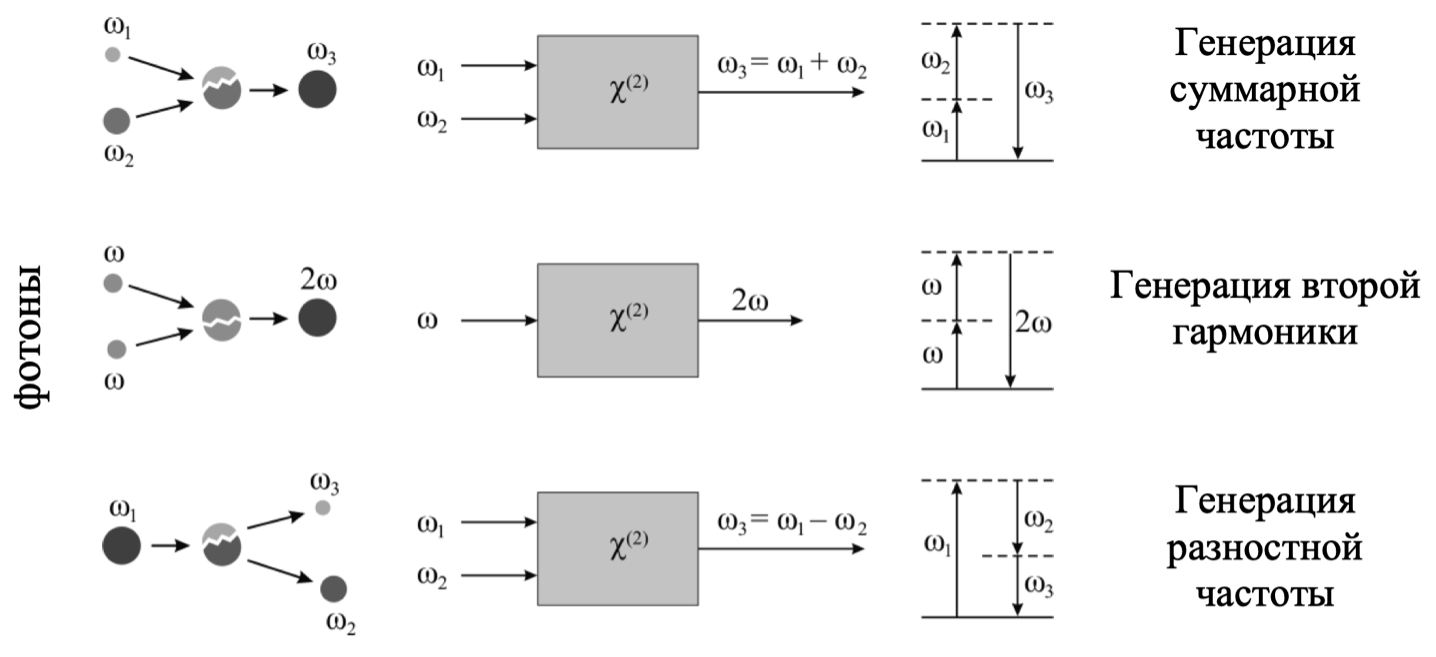
\includegraphics[width=0.7\linewidth]{images/shg.png}
	\caption{Схематическое представление нелинейно-оптических процессов второго порядка.}
	\label{sghPictr}
\end{figure}

\subsection*{Генерация третей оптической гармоники} 
Пусть на квадратично-нелинейную среду воздействует монохроматическое поле (\ref{shg:e(t)}) с частотой $\omega$. Тогда поляризация третьего порядка зависит от времени следующим образом:
\begin{equation}\label{thg}
P(t)^{(3)} = \chi^{(3)}E(t)^3 = \frac{1}{4}\chi^{(3)}A^3\cos(3\omega t) + \frac{3}{4}\chi^{(3)}A^3\cos(\omega t)
\end{equation}
То есть, происходит генерация третьей гармоники (THG) и переизлучение на исходной частоте (\textbf{самовоздействие света}) – см. рис. \ref{thg1}A, B. Поскольку, как правило, $\chi^{(3)}E^3 << \chi^{(2)}E^2$ то эффект THG в кубически-нелинейной среде очень мал, и на практике третью гармонику лазерного излучения получают путѐм последовательного удвоения частоты $\omega +  \omega \rightarrow 2\omega$, а затем сложения волн первой и второй гармоники: $\omega +  2\omega \rightarrow 3\omega$ в квадратично-нелинейной среде
\begin{figure}[h]
	\centering
	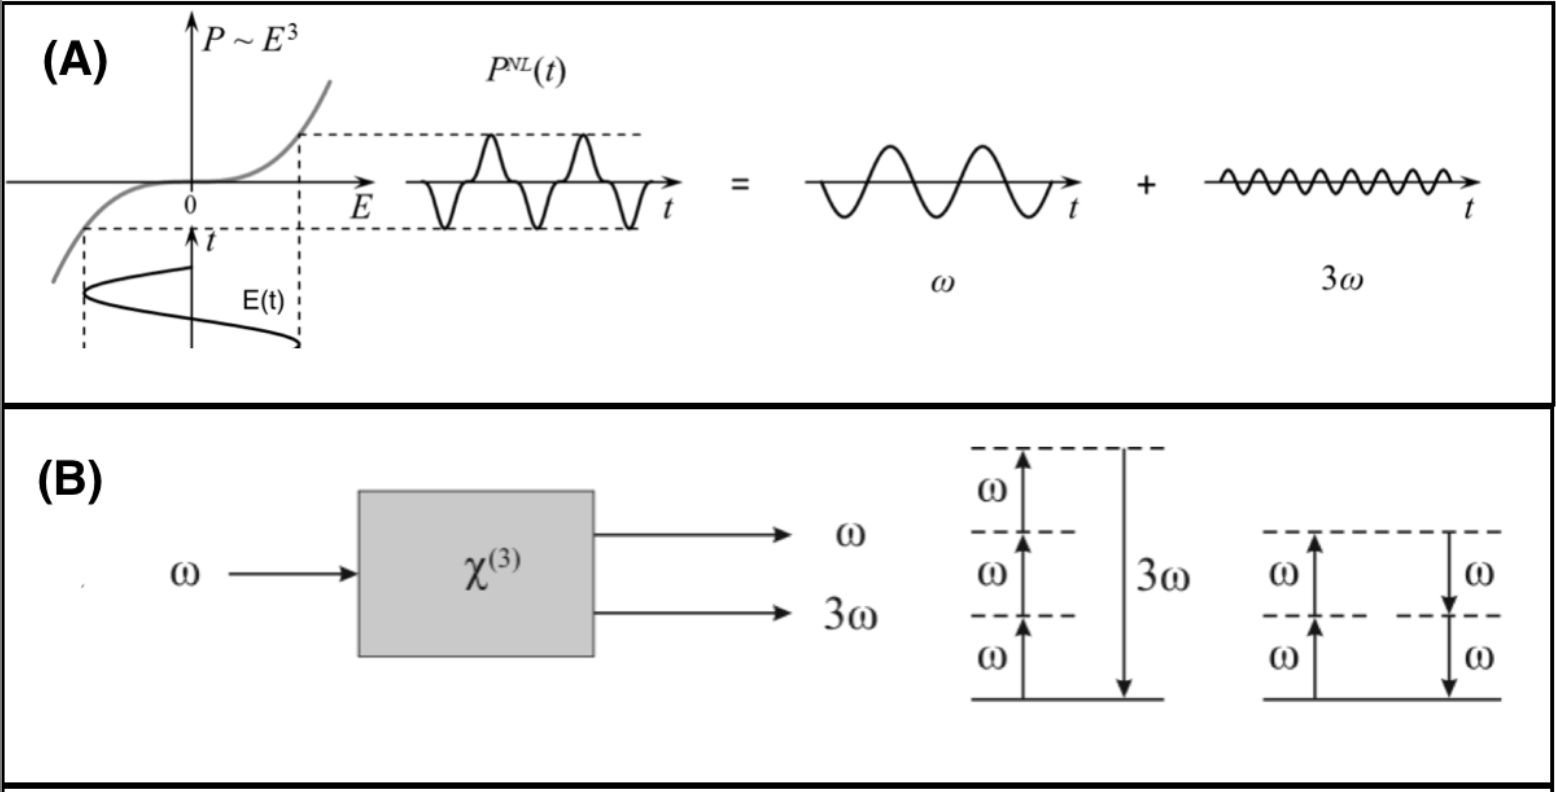
\includegraphics[width=0.8\linewidth]{images/thg.png}
	\caption{\textbf{(A)}: Поляризация среды третьего порядка. \textbf{(B-D)}: Схематическое представление нелинейнооптических процессов третьего порядка.}
	\label{thg1}
\end{figure}
В общем случае следует рассматривать оптическое поле как сумму трех волн: $E(t) = \frac{1}{2}(A_1e^{i\omega_1 t} + A_2e^{i\omega_2 t} + A_3e^{i\omega_3 t})$. Тогда будут возбуждаться колебания поляризации на всевозможных кобинациях частотат (пример некоторых процессовт рис. \ref{thg1}B-D, так-же см. ниже частотный смеситель\ref{mixerPictr1}). Второе слагаемое в правой части уравнения (\ref{thg}) описывает самовоздействие света. В простейшем случае можно показать, что оно сводится к изменению показателя преломления пропорционально интенсивности света: $n = n_0 + \gamma I$, где $ \gamma = \frac{12\pi^2 \chi^{(3)}}{n_{0}^{2}c} $. Если нелинейный коэффициент $\gamma > 0$, то показатель преломления в центре пучка, где интенсивность максимальна, больше, чем на периферии, поэтому пучок сходится к оси. Этот процесс называется \textbf{самофокусировкой}. В противном случае, при $\gamma < 0$, происходит \textbf{самодефокусировка} излучения. 


\section{Оптические резонансы полупроводниковых наноструктур}
\hspace*{2mm}
Наноразмерная оптика обычно связана с плазмонными структурами, сделанными из металлов, таких как золото или серебро. Основной проблемой наноплазмоники являются большие потери на нагрев металла и большие трудности в производстве. Недавние разработки в области наноразмерной оптической физики привели к появлению новой области нанофотоники, направленной на манипулирование оптически индуцированными резонансами Ми в диэлектрических и полупроводниковых наночастицах с высокими показателями преломления. Такие частицы предлагают уникальные возможности для уменьшения диссипативных потерь и большого резонансного усиления как электрического, так и магнитного полей. 
\\
\hspace*{2mm}
Эти недавние разработки тесно связаны с природой оптических резонансов структур и с методами, позволяющеми манипулировать этими резонансами. Для субволновой диэлектрической частицы с высоким индексом преломления, освещенной плоской волной, электрические (ED) и магнитные (MD) дипольные резонансы имеют сравнимую силу. Резонансный магнитный отклик возникает в результате связи внешнего света с круговыми токами смещения электрического поля, когда длина волны внутри частицы становится сравнимой с ее диаметром $d = 2R \approx \lambda/n$ где R - радиус частицы, n - показатель преломления, $\lambda$ - длинна волны.
\\
\hspace*{2mm}
Ожидается, что благодаря своим уникальным оптически индуцированным электрическим и магнитным резонансам нанофотонные структуры с высоким показателем преломления будут дополнять или даже заменять различные плазмонные компоненты. Кроме того, сосуществование сильных электрических и магнитных резонансов, их интерференция и резонансное усиление магнитного поля в диэлектрических наночастицах привносят совершенно новые функциональные возможности в простые геометрии, в значительной степени не исследованные в плазмонных структурах, особенно в нелинейном режиме или в приложениях оптоэлектронных устройств. 

\subsection{Ми резонансы в субволновых частицах}

 \begin{figure}[h!]
	\centering
	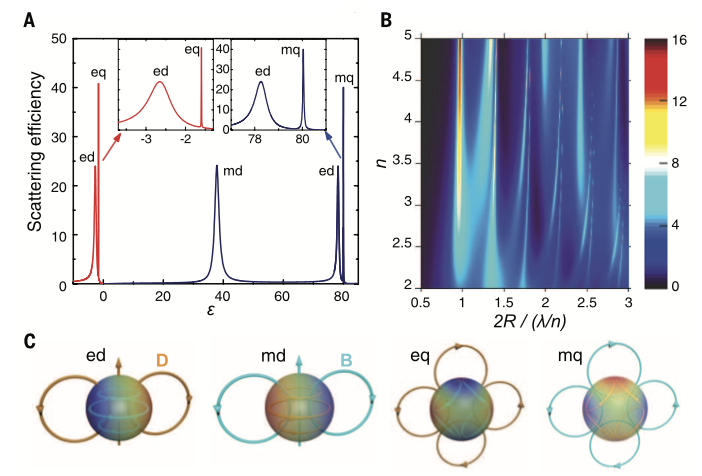
\includegraphics[width=0.7\linewidth]{images/fig1.png}
	\caption{Эффективность рассеяния (безразмерное отношение сечения рассеяния к геометрическому сечению частицы) в зависимости от диэлектрической проницаемости $\varepsilon$ (частицы без потерь, q = 0,5) для плазмонных ($\varepsilon$  < 0) и диэлектрических ( $\varepsilon$ > 0) материалов. Сокращения для резонансов: ed - электрический диполь; eq - электрический квадруполь; md - магнитный диполь; mq - магнитный квадруполь. \textbf{(B)} Эффективность рассеяния диэлектрической частицы без потерь (цветная шкала справа) как функция показателя преломления n и параметра размера. \textbf{(C)} Иллюстрация структур электрического и магнитного поля для различных электрических и магнитных резонансов, поддерживаемых сферической диэлектрической частицей.}
	\label{fig1}
\end{figure}
\hspace*{2mm}
Чтобы проиллюстрировать фундаментальные свойства рассеяния света наночастицами, рассмотрим случай сферической частицы, освещенной плоской волной, для которой существует точное аналитическое решение уравнений Максвелла. Согласно теории Ми \cite{absorbScattLight}, металлические и диэлектрические сферические частицы могут обладать сильными резонансами рассеяния (рис. \ref{fig1}A). В случае немагнитных материалов их свойства рассеяния зависят только от двух параметров: диэлектрической проницаемости $\varepsilon$  и размерного параметра q, который пропорционален отношению радиуса наночастицы R к длине волны света $\lambda$ ($q = 2\pi R/\lambda$). Различие между металлическими и диэлектрическими частицами заключается в знаке диэлектрической проницаемости, которая является отрицательной для металлов и положительной для диэлектриков. Небольшие металлические сферы (q < 1) создают только локализованные поверхностные плазмонные резонансы электрического типа:  дипольные, квадрупольные и т.д., в то время как их магнитный отклик остается практически незначительным из-за исчезающего поля внутри сферы (рис. \ref{fig1}А).  Чтобы воспроизвести "ощутимый" магнитный отклик от металлических структур, геометрия частицы должна другой. 
\\
\hspace*{2mm}
Например, резонатор с разрезным кольцом \cite{pendry1999magnetism} работает аналогично эффективной LC-схеме (то есть, цепи индуктор-конденсатор) с усилением магнитного поля в центре. Для диэлектрических частиц мы можем наблюдать как электрический, так и магнитный отклики сравнимых сил (рис. \ref{fig1}А). Резонансный магнитно-дипольный отклик является результатом взаимодейсвия входящего света с круговыми токами смещения электрического поля вследствие проникновения поля и замедления фазы внутри частицы. Это происходит, когда длина волны внутри частицы становится сопоставимой с диаметром частицы $2R \approx \lambda/n$ (рис. \ref{fig1}В). 
\\
Полевая структура четырех основных резонансных мод (MD -  магнитный диполь, ED - электрический диполь, MQ - магнитноый квадруполь,  EQ - электрический квадруполь) в диэлектрических частицах с высоким индексом приломления показана на рис. \ref{fig1}С. На длине волны магнитного резонанса возбужденная магнитно-дипольная мода диэлектрической сферы с высоким показателем может вносить основной вклад в эффективность рассеяния, превосходя моды других мультиполей на порядки величины.
\\
\hspace*{2mm}
Из теории Ми следует, что максимально достижимая эффективность рассеяния для конкретного многополярного возбуждения субволновой частицы зависит только от резонансной частоты, а не от типа материала \cite{schuller2009general}. Это говорит о том, что многие плазмонные эффекты, наблюдаемые при рассеянии света металлическими наночастицами, могут быть реализованы с помощью диэлектрических наночастиц с высоким индексом. На рисунке \ref{fig1}B показано масштабирование различных резонансов по отношению к показателю преломления n. При n > 2 все основные мультиполи хорошо определены, и их спектральные положения соответствуют фиксированному отношению длины волны внутри частицы к ее диаметру. Эффективность рассеяния всех мультиполей также увеличивается с ростом n \cite{articleOptSi}.
\\
\hspace*{2mm}
Сильные оптически индуцированные магнитные дипольные резонансы в диэлектрических наночастицах с высоким индексом могут быть достигнуты не только для сфер, но и для сфероидов \cite{articleDirVi}, \cite{optScatShper}, дисков и цилиндров \cite{multLightScat}, колец \cite{contrMagnModes} и многих других геометрий \cite{nearInfrMR}. Это обеспечивает важные возможности для создания разнообразных полностью диэлектрических наноструктур с желаемыми спектральными положениями резонансов. Изменяя геометрические параметры частиц, спектральные положения как электрического, так и магнитного дипольного резонансов могут настраиваться независимо, чередуя или перекрывая друг друга на одной частоте для простых геометрий \cite{optScatDeilectrHightIndex}.


\subsection{Наблюдение оптических магнитных резонансов в диэлектрических наночастицах.}


Кремниевые (Si) наносферы с размерами от 100 до 300 нм поддерживают сильные магнитные и электрические дипольные резонансы в видимой и ближней ИК областях спектра (рис. \ref{fig2}). 
 \begin{figure}[h]
	\centering
	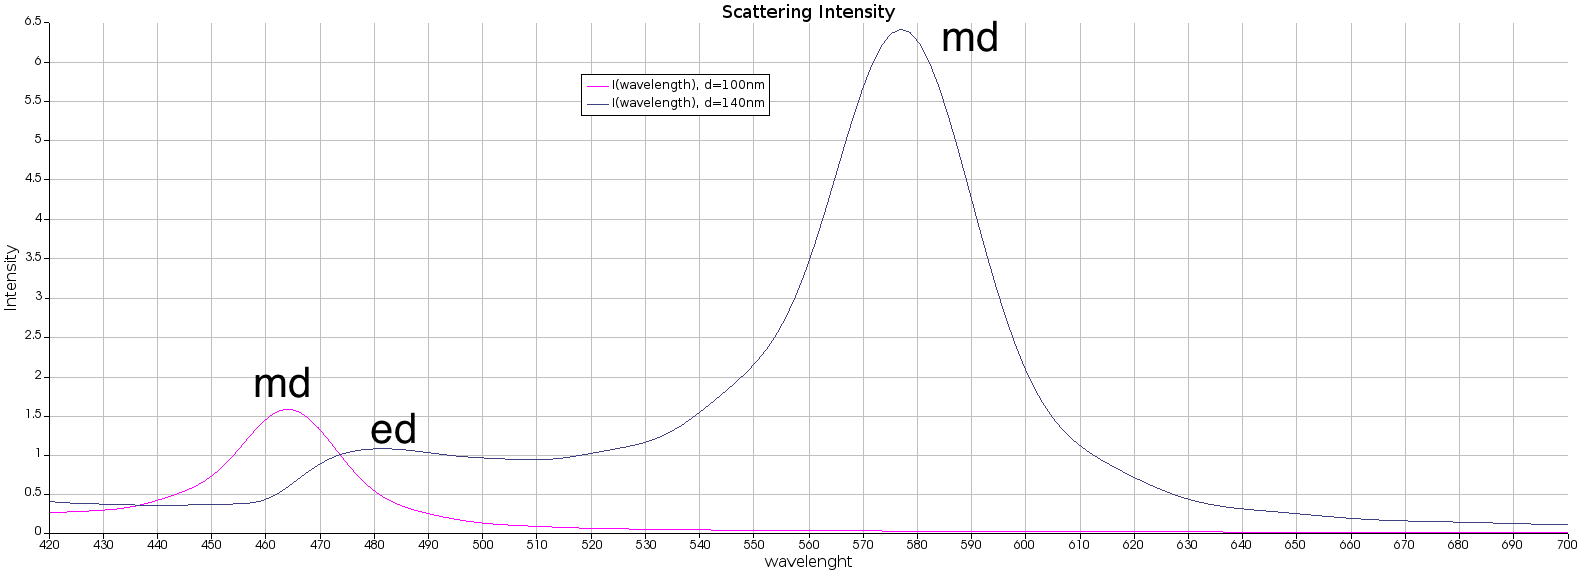
\includegraphics[width=0.7\linewidth]{images/graph1.png}
	\caption{Результат моделирования оптического магнитного отклика наночастиц кремния  диаметром 100 нм. (розовый график) и 140 нм. (синий график).  Сокращения для резонансов: ed - электрический диполь; md - магнитный диполь}
	\label{fig2}
\end{figure}
Экспериментальная демонстрация электрических и магнитных дипольных резонансов на видимых длинах волн впервые была представлена для сферических наночастиц Si, полученных с помощью фемтосекундной лазерной абляции на кремниевых и стеклянных подложках \cite{kuznetsov2012luk}. 
 \begin{figure}[h]
	\centering
	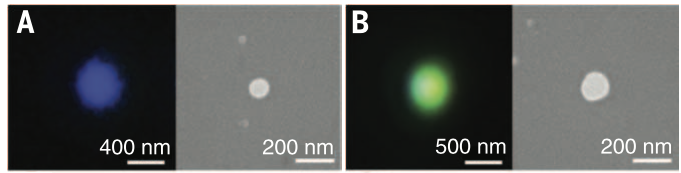
\includegraphics[width=0.7\linewidth]{images/fig2.png}
	\caption{ Изображения в темнопольном оптическом микроскопе (слева), изображения на сканирующем электронном микроскопе (SEM) (справа)  сферических наночастиц Si с приблизительными диаметрами 100 нм \textbf{(A)} 140 нм \textbf{(В)}} \cite{kuznetsov2012luk}
    \label{fig3}
\end{figure}
\hspace*{2mm}
Различные цвета, наблюдаемые на темнопольных микроскопах (рис. \ref{fig3}), соответствуют магнитным дипольным резонансам почти идеальных сферических наночастиц Si с размерами от 100 до 200 нм \cite{kuznetsov2012luk}.  Помимо кремния, полупроводники группы IV и группы III-V с показателями преломления выше 2 могут иметь аналогичные оптические свойства в зависимости от их поглощения и показателя преломления в конкретном диапазоне длин волн. Например, магнитные и электрические дипольные резонансы недавно были экспериментально обнаружены в нанодисках арсенида галлия (GaAs) в видимом спектре \cite{person2013demonstration}.


\section{Нелинейные оптические  резонансны диэлектрических наноструктур}
\hspace*{2mm}
Усиление в ближнем поле электрического и магнитного отклика в полностью диэлектрических наноструктурах может привести к новым нелинейным эффектам. В частности, генерация второй и третьей гармоник (SGH и THG), самоиндукция света и комбинационное рассеяние подвержены сильному ограничению в результате геометрических резонансов. Известно, что плазмонные резонансы, которые усиливают локальные электрические поля, усиливают нелинейно-оптические эффекты в металлических наноструктурах. В отличие от плазмоники, резонансы диэлектрических наночастиц с высоким индексом обеспечивают модовый объем, который может привести к более высокой эффективности преобразования.

\subsection*{Генерация третьей гармоники в наночастицах кремния, обусловленная магнитным откликом}
\hspace*{2mm}
Усиленная THG от нанодисков Si, демонстрирующих как электрический, так и магнитный дипольный резонансы, наблюдалась экспериментально \cite{shcherbakov2014enhanced} с помощью микроскопии и спектроскопии третьей гармоники, причем сигнал TH усиливался вблизи магнитного дипольного резонанса. Сканирующая электронная микрофотография нанодисков показана на рисунке \ref{nonliner:nanodisks}а. На рисунке \ref{nonliner:nanodisks1}b показан отрицательный логарифм спектра пропускания, полученный для этого образца с использованием установки, основанной на источнике белого света и ИК-спектрометре. Спектр нормализован по спектру смежной области образца.
\\
\hspace*{2mm}
Диски освещались интенсивным фемтосекундным лазерным импульсом с частотой $\omega$, близкой к магнитно-дипольному резонансу первого. В результате высокой восприимчивости кремния третьего порядка $\chi^3$ передаваемый сигнал содержал импульсы утроенной основной частоты $3\omega$. Поскольку сигнал третьей гармоники (TH) пропорционален кубу локальной напряженности поля, разумно ожидать значительного усиления процесса TH в нанодисках с их магнитными резонансами, возбуждаемыми фундаментальной волной. (рис. \ref{nonliner:nanodisks}). 
 \begin{figure}[h]
	\centering
	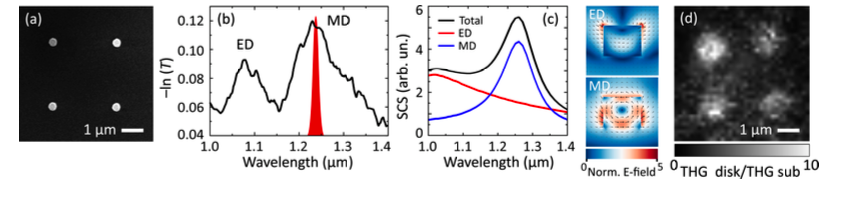
\includegraphics[width=1\linewidth]{images/fig4.png}
	\caption{Пространственно разделенные THG от отдельных нанодисков Si, усиленных магнитным резонансом. \textbf{(а)} Сканирующая электронная микроскопия изображения матрицы кремниевых нанодисков с d = 360 нм, h = 260 нм и p = 2,85 мкм. \textbf{(b)} Экспериментальный нормированный спектр пропускания образца (черный) со спектром импульса накачки, обозначенным красной областью. ED обозначает положение электрического дипольного резонанса, а MD - положение магнитного дипольного резонанса. \textbf{(c) }Рассчитанные спектры сечения рассеяния (SCS) нанодисков (черный), разложенных на электрические дипольные (красные) и магнитные дипольные (синие) вклады с соответствующими распределениями электрического поля. \textbf{(d)} Микроскопическое изображение образца, полученное с помощью сканирующего оптического микроскопа путем обнаружения сигнала THG при $\lambda = 413 \pm 5$ нм. Сигнал нормализуется сигналом, полученным при тех же условиях из области подложки. THG с усилением локального поля наблюдается на участках нанодисков по сравнению с подложкой между ними.}
	\label{nonliner:nanodisks1}
\end{figure}
\begin{figure}[h]
    \centering
	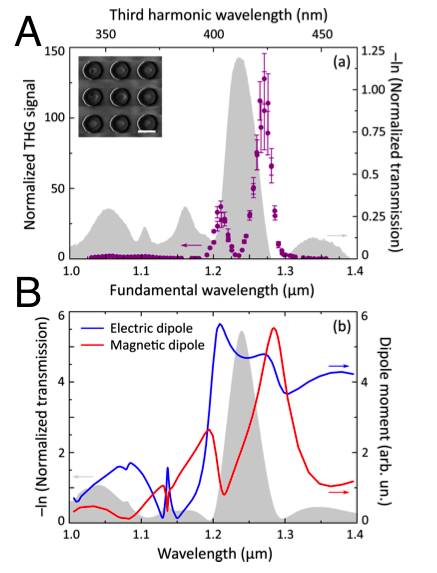
\includegraphics[width=0.9\linewidth]{images/fig3.png}
	\caption{\textbf{(А)}. THG-спектроскопия массивов нанодисков Si. Отрицательный логарифм нормированного спектра пропускания образца с p = 0,8 мкм, h = 220 нм и d = 0,5 мкм показан с серой областью, указывающей на резонанс при 1,24 мкм. Спектр THG образца, нормированный по спектру подложки, показан фиолетовыми точками. На вставке показано SEM-изображение фрагмента образца. Масштабная линейка  500 нм. \textbf{(B)} Моделируемый спектр пропускания основной длины волны через дискови и подложку, демонстрирующий хорошее согласие с наблюдаемой передачей в эксперименте. Наложенные синие и красные кривые дают величину электрических и магнитных дипольных моментов (соответственно). Двухпиковая структура каждого спектра дипольного момента вносит вклад в двухпиковый спектр THG в (A).}
	\label{nonliner:nanodisks}
\end{figure}
\hspace*{2mm}
Локализация поля в магнитном резонансе приводит к увеличению интенсивности гармоник на два порядка по отношению к неструктурированному объемному Si, при этом эффективность преобразования ограничивается только двухфотонным поглощением в подложке \cite{shcherbakov2014enhanced}. 


\section{Метаповерхности на основе резонансных металических наноструктур.}


\section{Метаповерхности на основе резонансных диэлектрических наноструктур.}
\hspace*{2mm}
Резонансные диэлектрические наночастицы также могут быть использованы для создания плоских однослойных решеток, известных как мета-поверхности \cite{yu2014flat}. Использование мета-поверхностей позволяет наблюдать различные резонансы  электрического и магнитно-оптического отклика в сочетании с низкими потерями тонкослойных структур. А следовательно, они демонстрируют многие полезные свойства мета-устройств. Одной из основных функций мета-поверхностей является контроль фазы отраженного и прошедшего света. Идея использования диэлектриков, структурированных в масштабе длины волны для управления волновым фронтом, активно обсуждалась два десятилетия назад \cite{lalanne1999design}. Подобные идеи также были реализованы в последнее время, чтобы достичь 2-фазного накопления.  На сегодняшний день эти решения обеспечивает наивысшую эффективность в режиме передачи до 90\%.
\\
\hspace*{2mm}
Другой подход к достижению фазового контроля был предложен в начале 2000-х годов, и он опирается на металлические или диэлектрические субволновые решетки с различной ориентацией для управления циркулярно поляризованным светом через геометрическую фазу Pancharatnam-Berry (PB). Недавняя работа, основанная на этом принципе, продемонстрировала плоские кремниевые линзы и аксиконы, работающие на видимых длинах волн (рис.  \ref{nonliner:matasurf1}А) \cite{lin2014dielectric}. Структура генерируется путем формирования рисунка наноантенн шириной 120 нм в пленку Si толщиной 100 нм. Его можно уменьшить по толщине относительно предыдущих элементов PB-фазы, используя резонансы в Si-структурах. Этот подход был далее распространен на высокоэффективную работу на видимых длинах волн с использованием прозрачного диоксида титана $(TiO_{2})$ в качестве материала мета-поверхности \cite{DiffLimFoc}. Фокусировка луча с эффективностью 66\%  была экспериментально продемонстрирована  на выбранных длинах волн в синей, красной и зеленой областях. В отличие от предыдущего примера, эта конструкция была достигнута при относительно большой высоте структур $(TiO_{2})$ (600 нм), что накладывает большие ограничения на нано-технологию.
\\
\hspace*{2mm}
Новым подходом к созданию диэлектрических мета-поверхностей является использование электрических и магнитных дипольных резонансов диэлектрических наночастиц для контроля фазы входящего света \cite{shalaev2015high}. Каждый из диполей способен сдвигать фазу от 0 до $\pi$ вблизи резонанса. Объединение отклика обоих диполей на одной и той же длине волны позволяет достичь полного покрытия \cite{decker2015high}. Такое перекрытие резонансов обеспечивает не только необходимые фазовые сдвиги, но и подавление обратного рассеяния, из-за первого условия Керкера.
 \begin{figure}[h!]
	\centering
	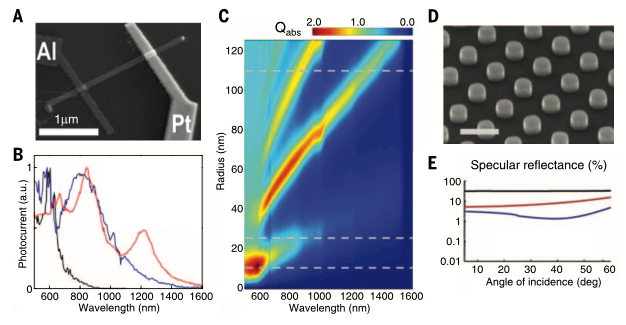
\includegraphics[width=0.6\linewidth]{images/fig5.png}
	\caption{ Нанофотонные устройства на основе полупроводниковых наноантенн. \textbf{(A)} Изображение фотодетектора с использованием оптически резонансной нано-проволоки Ge с асимметричными металлическими контактами. \textbf{(B)} Фототоковые спектры отдельных нанопроволок Ge с радиусами 10 нм (черный), 25 нм (синий) и 110 нм (красный). \textbf{(C)} Двумерный график рассчитанной эффективности поглощения как функции длины волны и радиуса нанопроволоки. Пунктирные серые линии указывают радиусы, для которых спектральный фототок показан в \textbf{(B). (D)} Изображение матрицы резонаторов Si, которая служит антибликовым покрытием на подложке Si \cite{spinelli2012broadband}. Масштабная линейка 1 мм. \textbf{(E)} Измерение зеркального отражения при 632 нм в зависимости от угла падения для непокрытой пластины Si (черного цвета), с антиотражающем покрытием Si3N4 толщиной 60 нм (красного цвета) и матрицы резонаторов Ми, как показано на \textbf{(D)} покрытый слоем $Si_3N_4$ толщиной 60 нм (синий) \cite{spinelli2012broadband}. }
	\label{nonliner:matasurf1}
\end{figure}
\\
\hspace*{2mm}
Такие конструкции концептуально аналогичны метаповерхностям Гюйгенса, предложенным в плазмонике \cite{pfeiffer2014efficient}, но они имеют гораздо более высокую эффективность пропускания из-за меньших потерь в прозрачных диэлектрических материалах. Недавно были продемонстрированы экспериментально мета-поверхности видимого диапазона на основе кремния с резонансным пропусканием более 85\%. Эти устройства имеют толщину всего 130 нм, что соответствует менее чем одной пятой длины волны в свободном пространстве, и способны контролировать волновой фронт света и выполнять отклонение луча с эффективностью передачи, близкой к 50\% (рис. \ref{nonliner:matasurf1}, В и С). Аналогичные концепции были также использованы для достижения эффективной генерации вихревого пучка (рис. \ref{nonliner:matasurf1}D). 
\\
\hspace*{2mm}
Помимо манипуляций с фазой пропускания, диэлектрические металические поверхности также могут быть использованы в качестве практически идеальных отражателей, превосходящих характеристики обычных металлических и диэлектрических зеркал \cite{moitra2015large},\cite{nearRefcLayer}.  Этот эффект возникает в результате когерентного взаимодействия магнитных или электрических диполей, возбуждаемых внешним излучением в каждой нано-частице. Недавний эксперимент продемонстрировал очень высокий коэффициент отражения (до 99,7\%) в ближней ИК-области спектра от плотного массива наночастиц Si \cite{moitra2015large}. Такое поведение с высоким коэффициентом отражения концептуально аналогично тому, которое наблюдалось ранее в высококонтрастных решетках с субволновой длиной. 
\\
\hspace*{2mm}
Мешающие электрические и магнитные диполи могут привести к явлениям, которые нельзя наблюдать с обычными диэлектриками или металлами. Одним из таких эффектов является поведение магнитного зеркала, когда диэлектрическая мета-поверхность действует как идеальный магнитный проводник, переворачивающий фазу падающего магнитного поля без влияния на фазу электрического поля \cite{optMagnMirr}. Другим примером является обобщенный эффект Брюстера. В отличие от обычного эффекта Брюстера, который ограничен p-поляризованным падением и углами выше $45^\circ$ (угол Брюстера ниже $45^\circ$ всегда сопровождается полным внутренним отражением под большими углами), обобщенный эффект Брюстера может быть достигнут для любой поляризации (как p, так и s) и любой угол падения (как ниже, так и выше $45^\circ$ без полного внутреннего отражения) (рис. \ref{nonliner:matasurf1}E). Оно возникает в результате интерференции электрических и магнитных резонансов в решетке и подавления их рассеяния в направлении отражения.

\subsection*{Возбуждение второй гармоники с использованием нарушенной симметрии III - V полупроводниковых метаповерхностей Фано}

\hspace*{2mm}Схема Фано-резонансной мета-поверхности показана на рисунке  \ref{nonliner:matasurf}а; структура состоит из группы ассиметричных  нанорезонаторов. Метаповерхность основана на маленьком кубе со сторона 300 нм, у которой вырезан один из углова. Во вставке на рисунке  \ref{nonliner:matasurf}а показан вид сверху и сканирующий электрон под углом $20^\circ$. Микроскопические (SEM) изображения изготовленной мета-поверхности, состоящий из нанорезонаторов с нарушенной симметриейс, расположены с шагом 470 нм. Размеры структуры был выбран больше, чем запрещенная зона GaAs, чтобы избежать поглощения накачки. Эта форма нанорезонатора приводит к смешению мод между поперечными и продольными дипольными модами света, что приводит к резонансу Фано с высокими значениями добротности. Эти резонансы могут наблюдаться как в спектре  пропускания так и в спектре отражения.

\begin{figure}[h!]
    \centering
	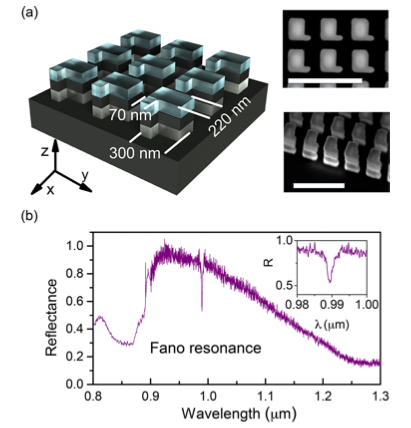
\includegraphics[width=0.5\linewidth]{images/fig6.png}
	\caption{Несимметричная мета-поверхность GaAs используется для создания резонансов Фано с высоким Q. \textbf{(а) }Схема фанорезонансной структуры мета-поверхности, основанная на кубе со стороной $\approx 300$ нм, который имеет угловой вырез. Верхняя часть вставки: изображение, полученное с помощью СЭМ сверху, изготовленной метаповерхности Фано. Вставка снизу: изображение, полученное с помощью СЭМ под углом $20^\circ$, изготовленной мета-поверхности Фано. Масштабная линейка соответствует 1 мкм. \textbf{(b)} Спектр отражательной способности мета-поверхности Фано, который обладает высоким Q-резонансом с шириной спектра $\approx$ 2 нм. Вставка представляет собой увеличенную область спектра отражения вокруг резонанса Фано. }
	\label{nonliner:matasurf}
\end{figure}

Резкий провал в спектрах отражения на рис. \ref{nonliner:matasurf}b при $\lambda_{F} \sim0,99$  мкм соответствует возбуждению резонанса Фано со спектральной шириной $\Delta\lambda_{F} \sim 2$ нм (добротность$\lambda_{F} /\Delta\lambda \sim 500$)). Численные расчеты показывают, что в идеальной наноструктуре усиление электрического поля внутри нанорезонатора при резонансе Фано достигает значения $|E|^2/|E_{0}|^2 \sim 500$. На рис. \ref{nonliner:matasurf2}A показана интенсивность сигнала второй гармоники, генерируемого  ассиметричной мета-поверхностью GaAs, когда мощность накачки поддерживалась постоянной, а длина волны накачки проходила через резонанс Фано. Спектр интенсивности SHG имеет узкий пик при $\sim$ 0,99 мкм который соответствует положению резонанса Фано в линейном спектре. Из-за локализации электромагнитного поля и увеличения его интенсивности Внутри нанорезонатора, возникающего на длине волны Фано-резонанса, сигнал SHG  (когда лазер накачки настроен на резонанс Фано) в  $\sim$ 300 раз сильнее по сравнению с нерезонансным случаем. На рисунке \ref{nonliner:matasurf2}A показан сценарий модификации нормализованного спектра SHG, когда длина волны несущей накачки отрегулирована относительно резонансной длины волны. Когда $\Delta\lambda_{F} = -10$ нм, перекрытия с резонансом Фано не происходит, и форма генерируемой второй гармоники близка к гауссовой .На рис. \ref{nonliner:matasurf2}B показано сравнение спектра SH, полученного на мета-поверхности GaAs при накачке на длине волны Фано-резонанса, и SH, генерируемого из неповрежденной области подложки GaAs. 
 \begin{figure}[h!]
	\centering
	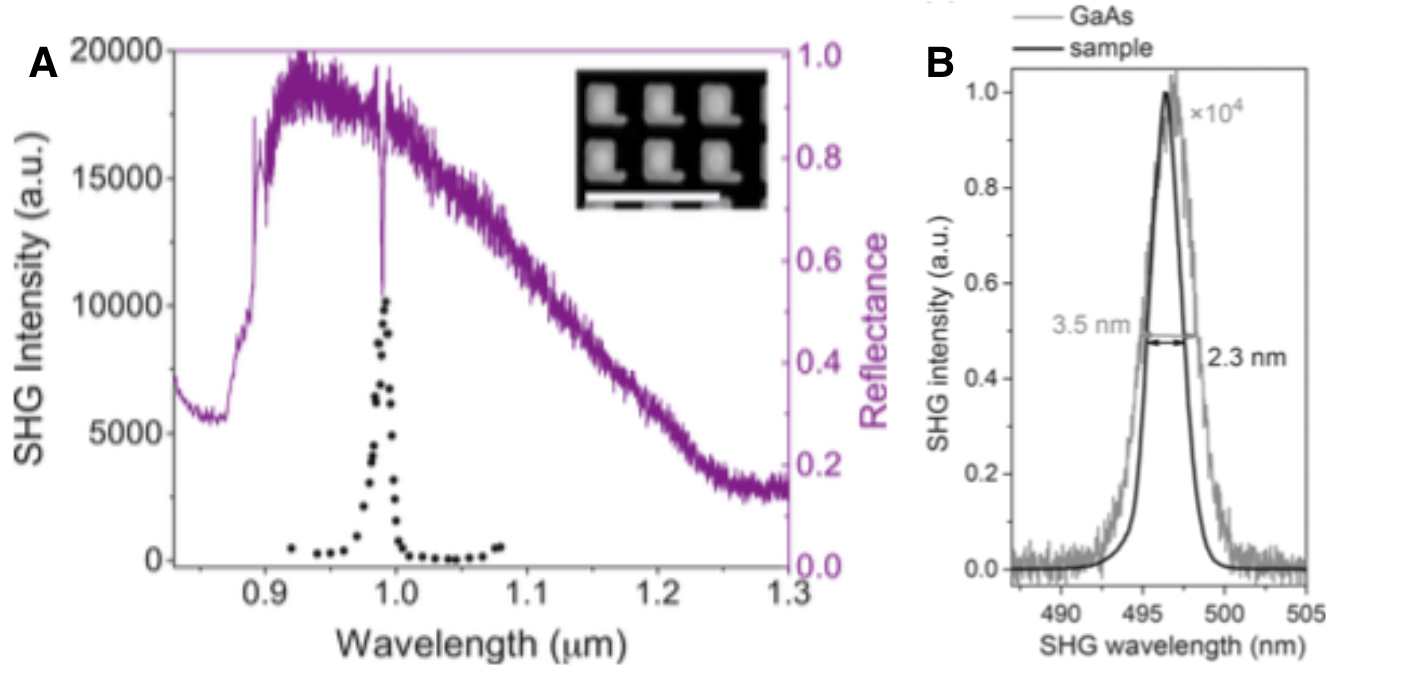
\includegraphics[width=0.7\linewidth]{images/fig7.png}
	\caption{\textbf{(A): }Генерация второй гармоники (SHG) на резонансной поверхности Фано. Точки: экспериментальная спектральная зависимость интенсивности SHG, демонстрирующая резонансно усиленную SHG на длинах волн резонанса Фано. Фиолетовый: линейный спектр отражения мета-поверхности Фано. Вставка: вид сверху образца SEM. \textbf{(B):} Сужение спектров SH, генерируемых мета-поверхностью Фано (черная линия), по сравнению с SH, генерируемым непокрытой подложкой GaAs (серая линия)}
	\label{nonliner:matasurf2}
\end{figure}


\subsection*{Использование диэлектрических метаповерхностей как широкополосный оптический частотный смеситель}
\textit{Частотный смеситель} - это нелинейное устройство, которое объединяет электромагнитные волны для создания волн на новых частотах. Эти устройства широко используются в  современных радиочастотных технологиях и в обработке микроволновых сигналов. Разработка универсальных частотных смесителей для оптических частот остается сложной задачей: такие устройства обычно полагаются на слабые нелинейные оптические процессы и, таким образом, должны удовлетворять условиям согласования фаз. Рассмотрим диэлектрическую метаповерхность на основе GaAs. Оптический смеситель на ее основе способен одновременно генерировать одиннадцать новых частот, охватывающих ультрафиолет и почти инфракрасный диапазоны. Нелинейности четного и нечетного порядка GaAs позволяют наблюдать генерацию \textit{второй гармоники}, \textit{третьей гармоники} и \textit{четвертой гармоники}, генерацию суммарной частоты, \textit{двухфотонную фотолюминесценцию}, вызванную поглощением,\textit{ четырехволновое и шестиволновое смешение}. Одновременному возникновению этих семи нелинейных процессов помогают комбинированные эффекты сильных внутренних нелинейностей материала, усиленных электромагнитных полей и ослабленных требований к фазовому согласованию. Такие ультракомпактные оптические смесители могут обеспечить множество применений в биологии, химии, зондировании, коммуникациях и квантовой оптике.
\\
\hspace*{2mm}
На рис. \ref{mixerPictr1}, а приведена схема генерации нелинейной частоты метасоверхностью GaAs, накачиваемой двумя лазерными лучами. Левая вставка на рис. \ref{mixerPictr1}а показывает изображение сканирующего электронного микроскопа (SEM) под углом $60^\circ$ метасоверхности GaAs, использованной в эксперементе. Метасоверхность состоит из периодической квадратной матрицы наноцилиндров диаметром $\sim 400$нм. Каждый наноцилиндр состоит из трех слоев: верхний надодиск из $SiO_x (\sim 300 $нм), средний нанодиск из GaAs толщиной $\sim 450$нм, в которым будет ограниченно электромагнитное поле, и нижний слой из $(Al_xGa_{1 - x})_20_3 \sim 400$нм с низким показателем преломления  для того чтобы отделить всесь цилиндр от подложки  с высоким индексом.
\\
\hspace*{2mm}
Резонансное усиление частот достигается за счет одновременного  возбуждения магнитных дипольных (MD) и электрических дипольных (ED) Ми-резонансов наноцилиндра GaAs \cite{liu2016iii}. В измеренном спектре отражатения (рис. \ref{mixerPictr1})b наблюдались максимумы при $\lambda_{ED} \sim 1,25$мкм и $\lambda_{MD} \sim 1,5$мкм, которые соответствуют возбуждению резонансов ED и MD. Это  подтверждается выполнением многополярным разложением полей рассеяния, а также моделированием профилей электрического поля (показано на вставках) для двух длин волн, которые соответствуют максимальному усилению электромагнитного поля внутри нанорезонаторов (1,246 мкм и 1,535 мкм).
\begin{figure}[h!]
	\centering
	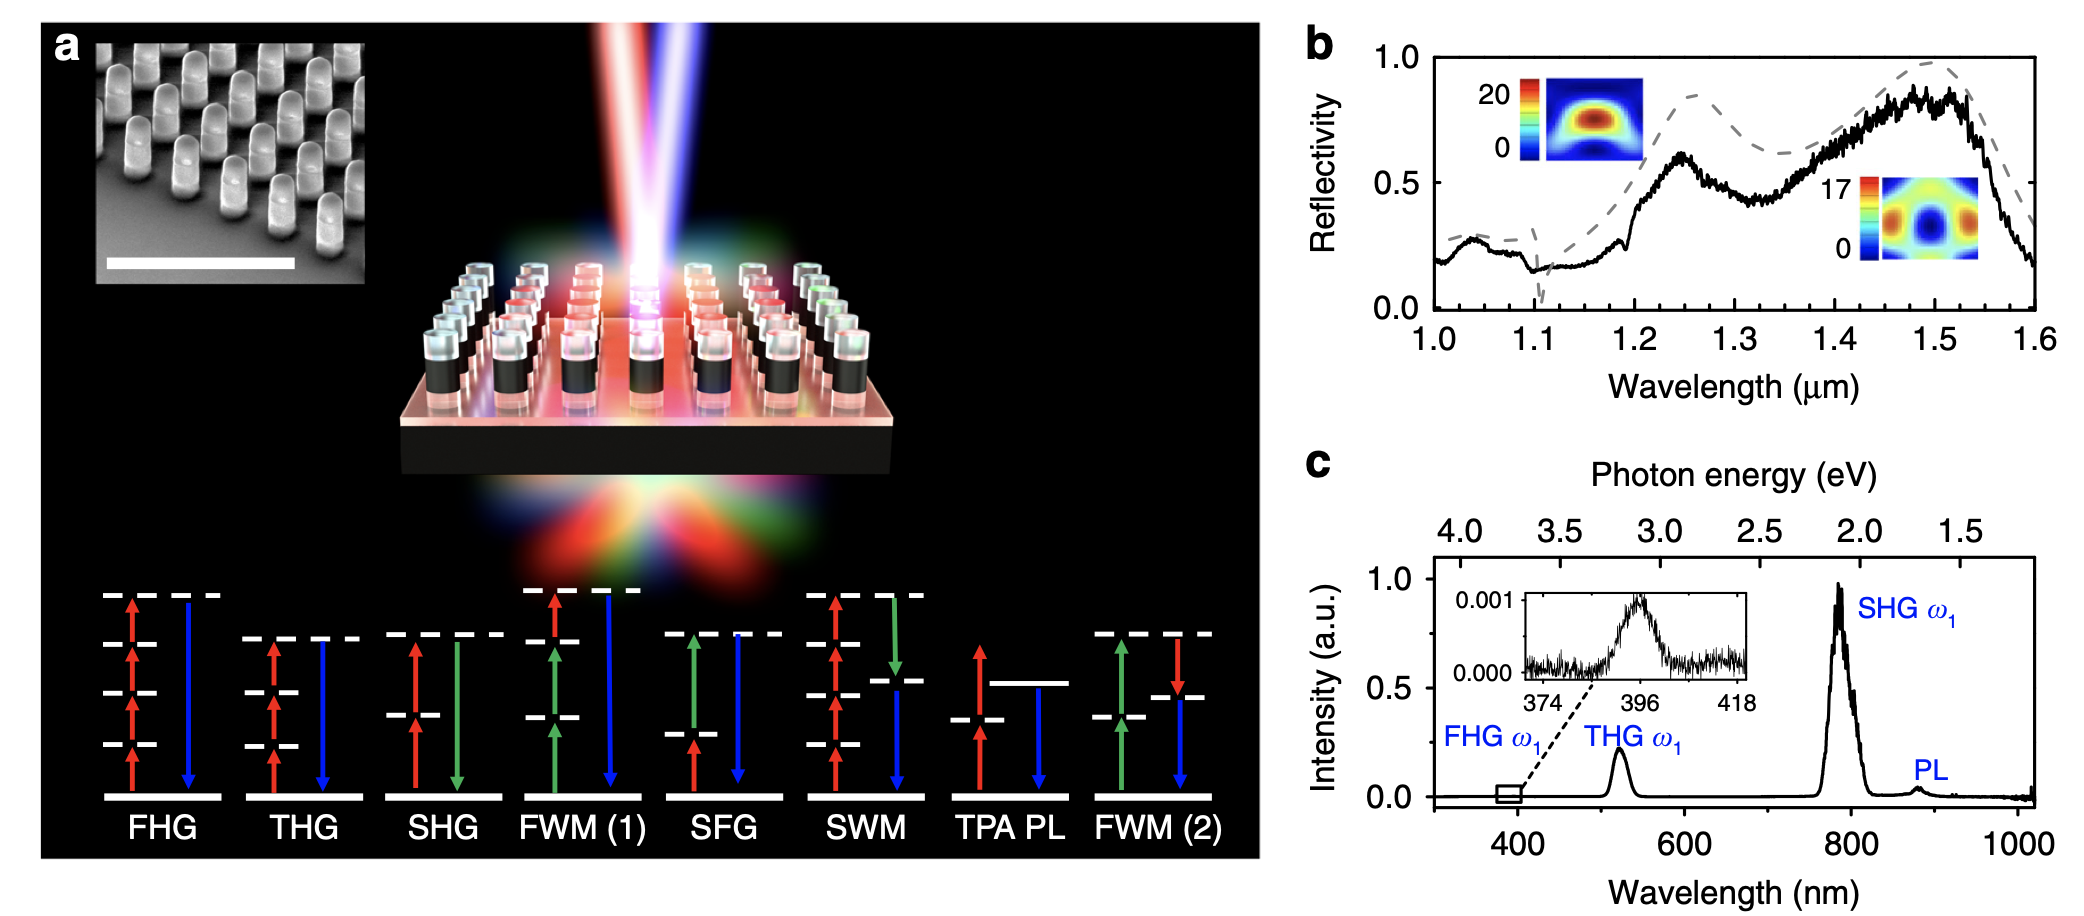
\includegraphics[width=0.7\linewidth]{images/mixer.png}
	\caption{Генерация новых частот с помощью метаповерхностью из  GaAs. Схема оптического метамиксера, состоящего из квадратной матрицы субволновых диэлектрических резонаторов. Два фемтосекундных ближних ИК-импульса накачивают метамиксер, и одновременно генерируется множество новых частот. Вставка: изображение сканирующего электронного микроскопа под углом 60 $^\circ$ поверхности GaAs. Масштабная линейка соответствует 3 мкм. Нижняя вставка: схематические энергетические диаграммы семи нелинейных оптических процессов, которые происходят одновременно в эксперементе: генерация второй гармоники (SHG), генерация третьей гармоники (THG), генерация четвертой гармоники (FHG), генерация суммарной частоты (SFG) фотолюминесценция, индуцированная двухфотонным поглощением (TPA PL), четырехволновое смешение (FWM) и шестиволновое смешение (SWM). \textbf{b} Измеренные (сплошная линия) и численно смоделированные (пунктирная линия) спектры отражения метаповерхности с двумя поперечными локальными распределениями электрического поля на длинах волн 1,246 мкм и 1,535 мкм, которые соответствуют максимальным усилениям электромагнитного поля внутри нанодиска GaAs. Спектры второй, третьей и четвертой гармоник, когда импульсы накачки $\lambda_1 \sim $1,57 мкм используются для возбуждения метамиксера. Врезка - это увеличение четвертой гармоники}
	\label{mixerPictr1}
\end{figure}
\textbf{Генерация гармоник в однолучевых экспериментах}. Сначала разберемся с генерацией гармоник метасоверхностью при накачке одним фемтосекундным лучом с длиной волны в близи MD резонанс ($\lambda_1 \sim$ 1,57 мкм) при средней мощности $\sim$ 4,5 мкВт. Рисунок \ref{mixerPictr1}с показывает вторую гармонику, третью гармонику и четвертую гармоника (вставка на рис. \ref{mixerPictr1}в), генерируемая метаповерхностью в $\lambda_{SHG} \sim$ 785 нм, $\lambda_{THG} \sim$ 523 нм, $\lambda_{FGH} \sim$ 393 нм соответственно. Излучение с центром при $\lambda_{PL} \sim$ 870 нм соответствует GaAs-фотолюминесценции (PL), возникающей при двухфотонном поглощении (TPA) накачки. Наблюдаемые гармоники лежат выше энергии запрещенной зоны GaAs и поэтому страдают от существенного поглощения материала. Эффективность преобразования намного выше, чем в недавно опубликованном отчете, который имеет высокую эффективность SHG с использованием специально подобранных плазмонных наноантенов. Тут надо заметить, что в работе \cite{wolf2015phased} были получены еще более высокие значения эффективности SHG из-за резонансной природы оптической нелинейности, созданной в трехуровневой системе с использованием межподзонных переходов в квантовых ямах. Эта конструкция не 
масштабируется за пределы нелинейностей 3-го порядка или до видимых и ближних ИК-длин волн; и при этом это не может использоваться, чтобы создать одновременные нелинейности более высокого порядка.
\\
\hspace*{2mm}
\textbf{Смешивание частот в двухлучевых экспериментах}. Посветим теперь на структуру вторым параллельным фемтосекундным лучом накачки, спектрально настроенный на $\lambda_2 \sim$ 1,24 мкм, чтобы перекрывать режим ED резонаторов. Когда два пучка накачки совпадают во времени, мы наблюдаем одиннадцать спектральных пиков в диапазоне от $\sim$ 380 до  $\sim$ 1000 нм (рис. \ref{mixerPictr2}а). Разделим сгенерированные сигналы на две группы. Первая группа, обозначенная синими метками, соответствует процессам генерации гармоник, а также PL, возникающим при двухфотонном поглощении. Каждый из процессов в этой группе опирается только на один пучок накачки. Напротив, вторая группа, обозначенная красными метками, соответствует процессам смешивания частот, которые требуют обоих импульсов накачки. Пять сигналов смешивания частот включают в себя: генерацию суммарной частоты $(\omega_1 + \omega_2)$ при $\lambda_{SHG} \sim$ 689 нм; три типа четырехволнового смешения $(2\omega_1 + \omega_2, 2\omega_2 + \omega_1, 2\omega_2 - \omega_1)$при $\sim$ 1000 нм, $\sim$ 472 нм и $\sim$ 434 нм соответственно; и шестиволновое смешение $(4\omega_1 - \omega_2)$ при $\lambda_{SWM} \sim$ 577 нм. Отметим, что амплитуда пика FWM $(2\omega_2 - \omega_1)$ как минимум в десять раз выше, чем у любого другого нелинейного процесса. Это объясняется гораздо меньшим поглощением ниже запрещенной зоны у  GaAs в отличие от сильного затухания, испытываемого другими сигналами. В целом спектры содержат одновременные вклады, возникающие в результате семи нелинейно-оптических процессов .
\\
Проверим  физическое происхождение процессов новых частот путем измерения выходных спектров для различных длин волн накачки и для разных мощностей накачки. Например, выход SFG идентифицируется по его энергии, совпадающей с суммой энергий фотонов двух пучков накачки $\omega_{SWG} = \omega_1 - \omega_2$, а также по линейной зависимости интенсивности от мощности одного накачки при мощности другого накачки поддерживается постоянным (рис. \ref{mixerPictr2}b, черная кривая). Аналогичным образом выполним измерения зависимости мощности для проверки процессов четырех- и шести-волнового смешения. Красная кривая на рис. \ref{mixerPictr2}b показывает квадратичную зависимость выхода FWM ($2\omega_2 - \omega_1$) от мощности накачки $\omega_2$, а на рис. \ref{mixerPictr2}в показана линейная зависимость интенсивности SWM от мощности накачки начастоте $\omega_2$. Чтобы дополнительно подтвердить процесс SWM, обе длины волны накачки были спектрально настроили. Результат отличного согласования между измеренным и рассчитанным местоположением пиков SWM показан на рисунке \ref{mixerPictr2}d. Для того, чтобы убедиться, что наблюдаемые нелинейные процессы усиливаются за счет накачки в диполярных резонансах Ми, были проведены аналогичные измерения смешивания частот как на непокрытой подложке GaAs, так и на других метаповерхностях GaAs с резонаторами разного диаметра, и, как и ожидалось, наблюдались значительно более низкие интенсивности сигналов \cite{liu2018all};  
\begin{figure}[h!]
	\centering
	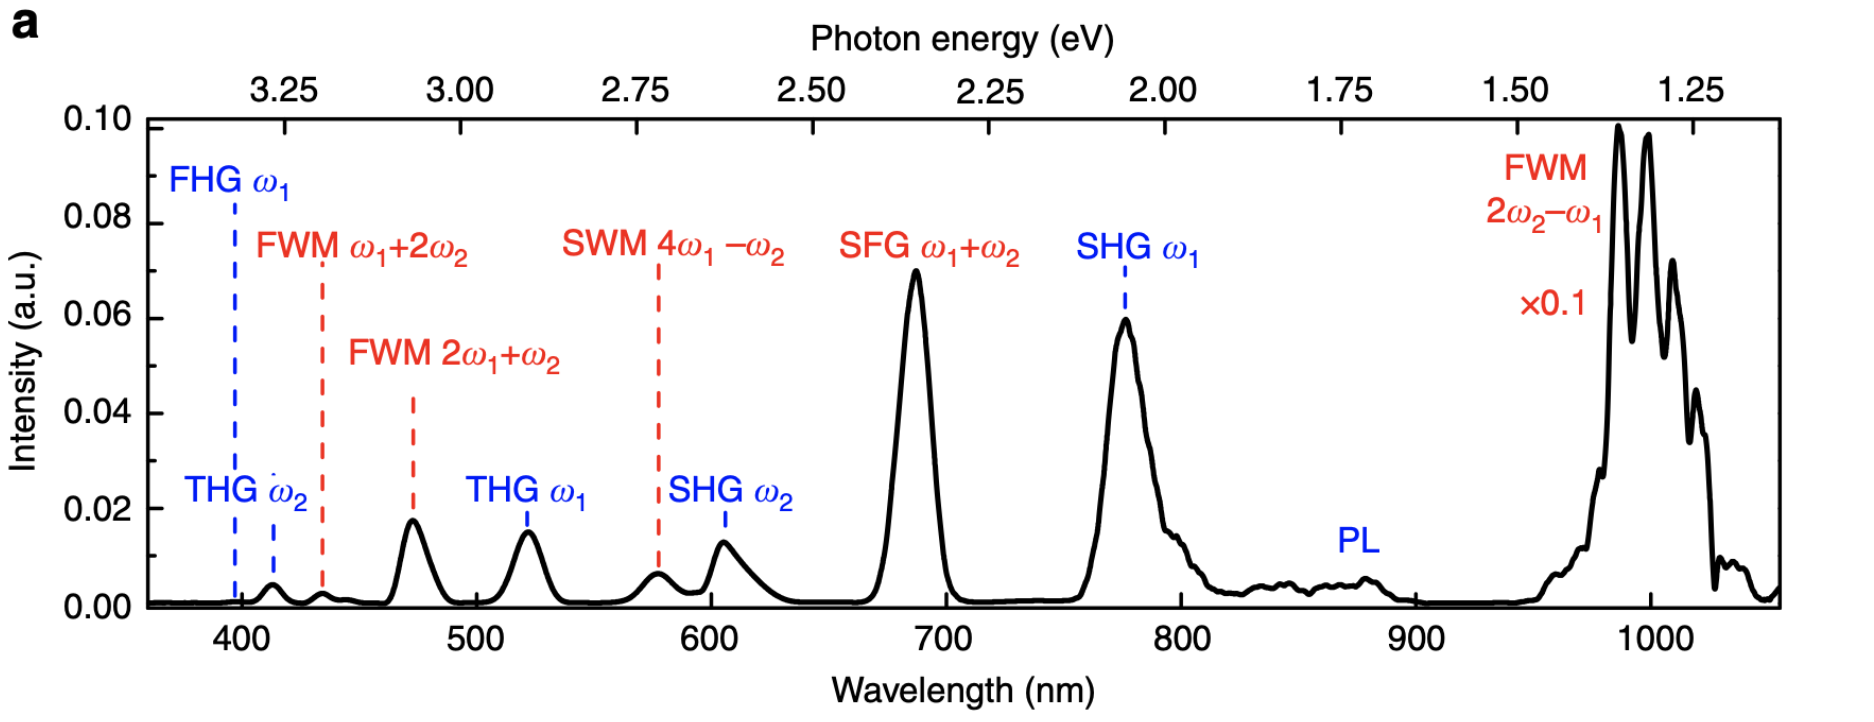
\includegraphics[width=0.8\linewidth]{images/mixer1.png}
	\caption{Смешивание частот в метасоверхности GaAs. Спектр, демонстрирующий одиннадцать нелинейно генерируемых пиков, возникающих в результате семи различных нелинейных процессов, когда два оптических луча с  $\lambda_2 \sim$ 1,24 мкм и  $\lambda_1 \sim$ 1,57 мкм используются для одновременной накачки метасоверхности GaAs. Синие метки указывают на процессы генерации гармоник и фотолюминесценции, возникающие в результате двухфотонного поглощения, для каждого из которых требуется только один луч накачки. Красные метки указывают на частоты, которое включает оба луча насоса. \textbf{b}, в Зависимость генерации суммарной частоты $(\omega_1 + \omega_2)$, четырехволнового смешения ($2\omega_2 - \omega_1)$ и шестиволнового смешения $(4\omega_1 - \omega_2)$ от мощности накачки $\omega_2$. Показаны экспериментальные  точки и теоретическое предсказание (черная линия для линейной подгонки и красная кривая для квадратичной подгонки). \textbf{d} Пять спектров, показывающих настройку нормированного шестиволнового смешивающего сигнала $(4\omega_1 - \omega_2)$, когда длины волн накачки спектрально настроены на $\lambda_2 \sim$ 1248,7 нм,  $\lambda_1 \sim$ 1557,5 нм (черная кривая); $\lambda_2 \sim$ 1234,8 нм, $\lambda_1 \sim$1558,6 нм (красная кривая); $\lambda_2 \sim$1211,6 нм, $\lambda_1 \sim$ 1558,9 нм (синяя кривая); $\lambda_2 \sim$ 1234,9 нм, $\lambda_1 \sim$ 1581,2 нм (зеленая кривая); и $\lambda_2 \sim$ 1233,7 нм, $\lambda_1 \sim$1600,4 нм (пурпурная кривая). Стрелками обозначены теоретически ожидаемые частоты для рассматриваемого шестиволнового процесса смешения}
	\label{mixerPictr2}
\end{figure}
\\
Экспериментальная демонстрация семи разных нелинейныхоптические процессы, происходящие одновременно в GaAs метасоверхности может быть использована для реализации ультракомпактных оптических смесителей. Видно, что нечетные нелинейные процессы высокого порядка могут генерировать гармоники высокого порядка, являющиеся основой генерации аттосекундных импульсов. Кроме того, что эти мета-поверхности могут быть оптимизированы для других нелинейных процессов смешивания, таких как генерация разностной частоты $\omega_{DFG} = \omega_1 - \omega_2$. Это позволило бы создавать фемтосекундные импульсы, охватывающие среднюю инфракрасную область спектра. 



































